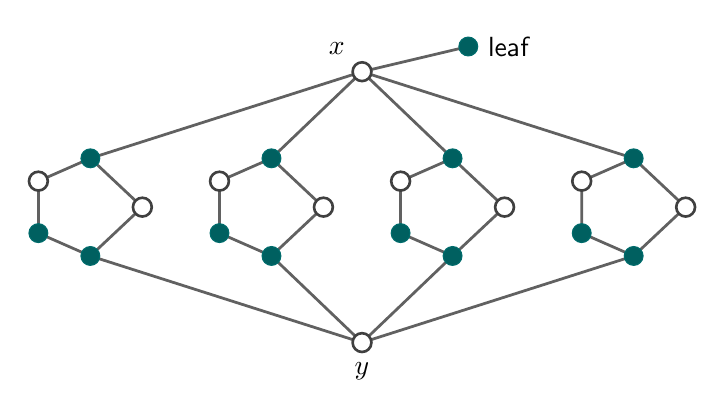
\begin{tikzpicture}[x=1cm,y=1cm,font=\sffamily,
 edge/.style={line width=1.0pt,draw=black!62},
 pick/.style={circle,draw=teal!85!black,fill=teal!75!black,inner sep=0pt,minimum size=6.8pt},
 skipv/.style={circle,draw=black!75,fill=white,line width=.95pt,inner sep=0pt,minimum size=6.8pt}]
\coordinate (x) at (0,1.72); \coordinate (y) at (0,-1.72);
\coordinate (l) at (1.35,2.04);
\foreach \i/\dx in {1/-3.45,2/-1.15,3/1.15,4/3.45}{
  \begin{scope}[xshift=\dx cm]
    \coordinate (a\i) at (0,.62); \coordinate (b\i) at (.66,0);
    \coordinate (c\i) at (0,-.62); \coordinate (d\i) at (-.66,-.33);
    \coordinate (e\i) at (-.66,.33);
  \end{scope}
  \draw[edge] (x)--(a\i)--(b\i)--(c\i)--(d\i)--(e\i)--(a\i);
  \draw[edge] (c\i)--(y);
  \foreach \letter in {a,c,d} \node[pick] at (\letter\i) {};
  \foreach \letter in {b,e} \node[skipv] at (\letter\i) {};
}
\draw[edge] (x)--(l);
\node[skipv,label=above left:{$x$}] at (x) {};
\node[skipv,label=below:{$y$}] at (y) {};
\node[pick,label=right:{leaf}] at (l) {};
\end{tikzpicture}
